\documentclass[a4paper]{article}
% Fixing nice colours 
\usepackage[dvipsnames, svgnames]{xcolor}
% Placing figures in parallel
\usepackage{graphicx, wrapfig} 
% Basic math 
\usepackage{amsmath, amssymb}
\usepackage{floatflt} %f�r inkapslade bilder.
\usepackage{fancyhdr}
\usepackage[top=3cm, bottom=3cm,inner=3cm, outer=3cm]{geometry}	
% Create cover page 
\usepackage{eso-pic}
\usepackage[utf8]{inputenc}
\usepackage[swedish, english]{babel}
\usepackage[numbers]{natbib}
\usepackage[toc,page]{appendix}
% Fixing paragraphs 
\setlength{\parskip}{5.5pt}  % x pt = hopp mellan stycken
\setlength{\parindent}{0pt} % 0 pt  = indrag
% Figurtexter 
\usepackage[format=plain, labelfont={bf}, textfont=it]{caption}  
 % Tillåter bilder att läggas bredvid varandra med kommandot \subfigure
\usepackage{subcaption}
\usepackage{enumitem}
\usepackage{wasysym}
% For inserting links
\usepackage{hyperref} 
% For inserting trees
\usepackage[linguistics]{forest}   

\begin{document}\thispagestyle{empty}

\pagenumbering{gobble} 

\newcommand{\HRule}{\rule{\linewidth}{0.5mm}} % Defines a new command for the horizontal lines, change thickness here

\begin{center} % Center everything on the page
 
%----------------------------------------------------------------------------------------
%	HEADING SECTIONS
%----------------------------------------------------------------------------------------

\textsc{\LARGE Chalmers University of Technology}\\[1.5cm] % Name of your university/college
\textsc{\Large Advanced Bioinformatics, BBT015}\\[0.5cm] % Major heading such as course name

\textsc{\Large }\\[0.5cm] %
%----------------------------------------------------------------------------------------
%	TITLE SECTION
%----------------------------------------------------------------------------------------

\HRule \\[0.8cm]
{ \huge \bfseries Project Report on Replication of a Study 
 }\\[0.8cm] 
\Large \bfseries Transcriptional Landscape of a bla$_{KPC-2}$ Plasmid and Response to Imipenem Exposure in Escherichia coli TOP10
% Title of your document
\HRule \\[0.8cm]


 
%----------------------------------------------------------------------------------------
%	AUTHOR SECTION
%----------------------------------------------------------------------------------------

\begin{minipage}[t]{0.5\textwidth}
\begin{flushleft} \large
\emph{Authors}\\
\bigskip
% Your name
Emma Andersson\\
Andrea Clausen Lind\\
Martina Hermanova Billstein\\
Sebastian Persson

\end{flushleft}
\end{minipage}
~
\begin{minipage}[t]{0.4\textwidth}
\begin{flushright} \large
\emph{Supervisors}\\
\bigskip
% Supervisor's Name
Aleksej Zelezniak\\
Filip Buric
\end{flushright}
\end{minipage}\\[2cm]

%----------------------------------------------------------------------------------------
%	DATE SECTION
%----------------------------------------------------------------------------------------
\vfill % Fill the rest of the page with whitespace

{\large \today}\\[2cm] 



\end{center}

\newpage

%ABSTRACT
\section*{Abstract}
%\textcolor{red}{Får man ha källor i abstract? \\"It is adviced that researchers refrain from citing the works of others when writing abstracts."\\Should be 100-300 words, alternativt 200-250 ord?. Current count: 158}

A critical aspect of any scientific study is to strengthen the reliability of the conclusions stated in the study. In order to do so, the study should be reproducible, not only by its original authors, but by other independent studies. In this study, the data analysis of an RNA-seq study with corresponding data has been reproduced and then compared to the results in the original study. The chosen study, \textit{Transcriptional Landscape of a bla$_{KPC-2}$ Plasmid and Response to Imipenem Exposure in Escherichia coli TOP10}, aimed to analyse how gene expression in a plasmid-induced \textit{E. coli}-strand is affected by the antibiotic Imipenem \cite{jousset2018transcriptional}. Not considering the plasmid, the results from this replicational study were found to be similar enough to the original findings, in E.coli. Nevertheless, the exact same results were not obtained. Whilst the results from the plasmid seemed to be similar regarding the fold change of the expression of the most significant genes, this could not be confirmed due to missing information on the gene names that were given in the original study. Therefore, the study was concluded not to be completely reproducible.


%Detta var originalslutet som är ersatt fr.o.m. "Not considering...."  
%The results from this replicational study were found to be similar to the original findings, although the exact same results were not obtained. The original study was thus found to be reproducible, with the exception of missing data on the gene names for the plasmid in the replicational study. 

\newpage

%%%%%%%%%%%%%% Table of content %%%%%%%%%%%%%%%
\pagebreak
\tableofcontents
\pagebreak
\pagenumbering{arabic} 

%%%%%%%%%%%%%%%%%%%%%%%%%%  The text begins here %%%%%%%%%%%%%%%%%%%%%%%%%%%%



\newpage
\section{Introduction}
%http://journals.plos.org/ploscompbiol/article?id=10.1371/journal.pcbi.1005619

%Why it is important to be able to reproduce this article
The minimum requirement for an article in research to be believable is reproducibility \cite{goodman2016does,peng2011reproducible}. For a study to be reproducible, each step has to be described in enough detail to enable someone else to completely repeat the same procedure and, given the same data and material, obtain the same results \cite{goodman2016does}.

%Aim
Here, we aim to reproduce the results of the differential gene expression analysis in the study ”Transcriptional Landscape of $bla_{KPC-2}$ Plasmid and Response to Imipenem Exposure in \textit{Escherichia coli} TOP10” \cite{jousset2018transcriptional}. In the study a plasmid called pBIC1a, carrying the multi-resistance gene $bla_{KPC-2}$ as well as other genes (only two more related to antibiotic resistance), was introduced in \textit{E. coli} K-12 sub-strain DH10B. The plasmid had been isolated from \textit{Klebsiella pneumonia} in which it seemed connected to the rapid spread of the bacteria. The purpose of the study was to identify the plasmid sequence, to gain understanding of basal gene expression from the plasmid and genome, as well as in the transcriptional changes at exposure to imipenim, a broad spectrum antibiotic \cite{clissold1987imipenem}. Of the different procedures in the study, we aim to reproduce the alignment of transcriptomic data to the \textit{E.coli} genome and the plasmid sequence, as well as reproducing the differential gene expression analysis  \cite{jousset2018transcriptional, rosinski2015single}.

%Outline of the article
 In the article six samples were analysed, the first three samples (sample 1-3) act as control and have not been exposed to  imipenem, while the last three samples (sample 4-6) have been exposed to imipenem for 10 minutes before extraction of RNA. Results showed that of the plasmid genes, nine out of 234 were upregulated when at imipenem exposure. However, none of these genes were the antibiotic resistance genes. The remaining genes were expressed at a lower level, with the most expressed ones were related to antibiotic resistance, plasmid replication and conjugation, or connected to mobile elements in the plasmid. Looking at the \textit{E.coli} there was a bigger change in expression. Of all the native \textit{E. coli} genes, 1563 out of 4550 genes were differentially expressed as a response to the imipenem exposure.

%Scientific justification of our claims and findings --> Bakgrund med källor till grejer vi vill förklara 


To reproduce these results the method described in the paper was followed as closely as possible. In the study, Bowtie version 0.12.7 was used to align the RNA-seq reads to the reference sequences. Hence, this of Bowtie version 0.12.7 was downloaded and used to reproduce the study as well. The differential gene expression analysis was performed using R version 3.5.2, whilst the version used in the original study was 3.3.1. Using an older version would have resulted in problems regarding DESeq, as this function relies on other functions that have to be compatible. Thereby this was omitted.

%This means that the versions of functions used for the analysis were different as well. Downloading the older versions were considered, but for DESeq this would have resulted in problems, as this function relies on other functions that have to be compatible. Thereby this was omitted.


As for the results of the study reproduction it was partially successful. Some differences were found in terms of number of total gene numbers and annotation of the plasmid genes was unsuccessful, making it hard to compare these results. However, the significance and expression level of genes in the \textit{E.coli} were found to be similar and the expression levels of the plasmid genes seem to match the genes in the paper, even if the identity of the respective genes could not be identified. Given the requirement of reproducibility is the possibility of recreating the same results given the same data, the similarity in results is insufficient. 


















\newpage
\section{Method} 
\subsection{Data description retrieval}

The RNA-seqeunce data was retrieved from \href{https://www.ebi.ac.uk/arrayexpress/}{\color{MidnightBlue} \underline{ArrayExpress}}, association number E-MTAB-7190. In the study, sequencing of the data was performed using Illumina HiSeq 2500 in singe-read mode with 50 cycles, for more information regarding the sample data see the original paper \cite{jousset2018transcriptional}. The reference genome, and associated gff3-file, for the \textit{E. coli}  K-12 sub-strain DH10B was downloaded from NCBI-nucelotide database, accession number \href{https://www.ncbi.nlm.nih.gov/nuccore/CP000948.1}{\color{MidnightBlue} \underline{CP000948.1}}. The reference genome, and associated gff3-file, for the pBIC-1a plasmid was also downlaoded from NCBI-nucleotide database, accession number \href{https://www.ncbi.nlm.nih.gov/nuccore/CP022574}{\color{MidnightBlue} \underline{CP022574}}. 

 %In total the data consists six samples of \textit{E.coli} K-12 sub-strain DH10B transformed with the pBIC-1a plasmid. The first three samples (sample 1-3) act as control and have not been exposed to  imipenem, while the last three samples (sample 4-6) have been exposed to imipenem for 10 minutes before extraction of RNA.

\subsection{Alignment using bowtie-0.12.7}

Bowtie-0.12.7 \cite{langmead2009} was downloaded from \href{https://sourceforge.net/projects/bowtie-bio/}{\color{MidnightBlue} \underline{SourceForge}}. All bowtie functions used were from this version.

 Indexes were created for the genome of E.coli TOP10 and the 
 plasmid pBIC1a using bowtie-build. Bowtie was then used to align RNA-seq samples 1-6 to the reference sequences, using the indexes. Samples were not filtered prior to alignment, and no filtering was performed of the alignments. Samtools (version 1.9-97-g4a51966) was used to convert the sam-file output from bowtie to bam-file format \cite{li2009sequence_sam_tools}. The bam-files were not sorted as there was no need for this.    
 
\subsection{Differential analysis}

In order to perform differential analysis a count matrix (rows corresponding to genes and columns to samples) was generated from the aligned \textit{E. coli} and the pBIC-1a plasmid data. The count matrix was created using Rsamtools (version 1.34.1), GenomicFeatures (version 1.34.3) and GenomicAlignments (version 1.18.1) in R (version 3.5.2) \cite{lawrence2013software_gen_align, morgan2016rsamtools}. The union mode was chosen for performing the counting with the \textit{summarizeOverlaps}-function, meaning that reads overlapping more than one feature (gene) were discarded. 

The differential analysis was performed using the DESeq2-package (version 1.22.2), which tests for significance using a negative-binomial model of the counts \cite{love2014moderated_DESeq2}. The p-values were adjusted by the Benjamini–Hochberg procedure which controls the false-discovery rate (fdr), and a fdr-cut off at 0.05 was chosen \cite{benjamini}. For the PCA-plot the data was normalised by the vst-procedure in DESeq2 \cite{love2014moderated_DESeq2}. All the code used to perform the analysis can be found at the projects GitHub \href{https://github.com/sebapersson/Project_BBT015}{\color{MidnightBlue} \underline{repository}}. 

\newpage
\section{Results}
%----------------------------------------------------------------------------------------
%	E.coli SECTION
%----------------------------------------------------------------------------------------
\subsection{\textit{E. coli}}
The original study found 1563 significantly differentially expressed genes in \textit{E. coli}. PCA-plots of the first principal component against the second and third principal component, from the study, are presented in figure \ref{fig:orig_study_figures}a. The first principal component explains the majority of the variance and clearly separates the case samples and controls. Figure \ref{fig:orig_study_figures}b presents a volcano plot of the studied genes, where genes to the right in the plot have been up-regulated in the case samples compared to the controls, while genes to the left have been down-regulated \cite{jousset2018transcriptional}.

\begin{figure}[h!]
    \centering
    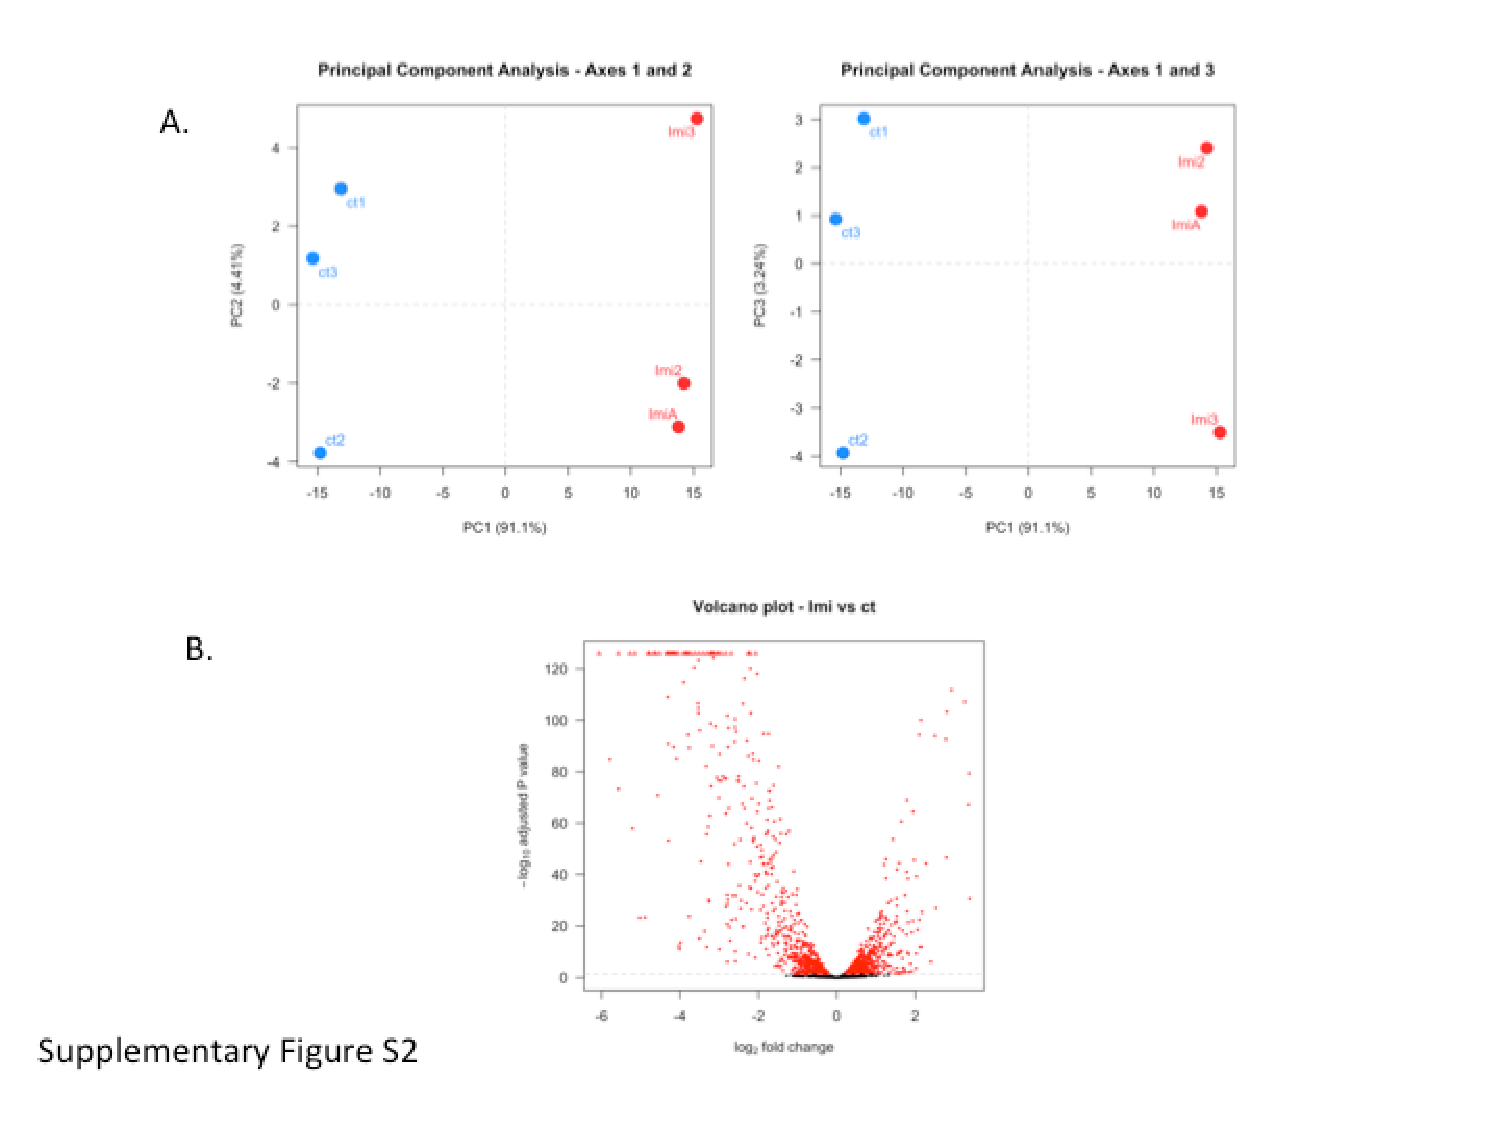
\includegraphics[scale=0.6]{Figures/Orig_study_figures.pdf}
    \caption{The figures presented in the the original study by Jousset et al. A. represents the PCA-plot for \textit{E. coli} samples and B. is the volcano plot for studied expressed genes in \textit{E. coli} \cite{jousset2018transcriptional}.}
    \label{fig:orig_study_figures}
\end{figure}

 % PCA #2
In this study, a PCA-plot was created based on the normalised data of E.coli genes and is presented in figure \ref{fig:pca_volc_E_coli}a. The first principal component explains 89\% of the variance and clearly separates the controls from the case samples. The PCA-plot is similar to the plot in the original study.

% Volcano #4or3
The genes studied in the differential expression analysis are plotted in the volcano plot, as seen in figure \ref{fig:pca_volc_E_coli}b. The significantly differentially expressed genes (adj p-value$<$0.05) with absolute $\mathrm{log}_2$ fold-change $\geq2$ are represented in blue and are of particular interest since their gene regulation has changed remarkably. The volcano plot is similar to the plot in the original study.

\begin{figure}[ht]
    \centering
    \begin{subfigure}{0.47\textwidth}
        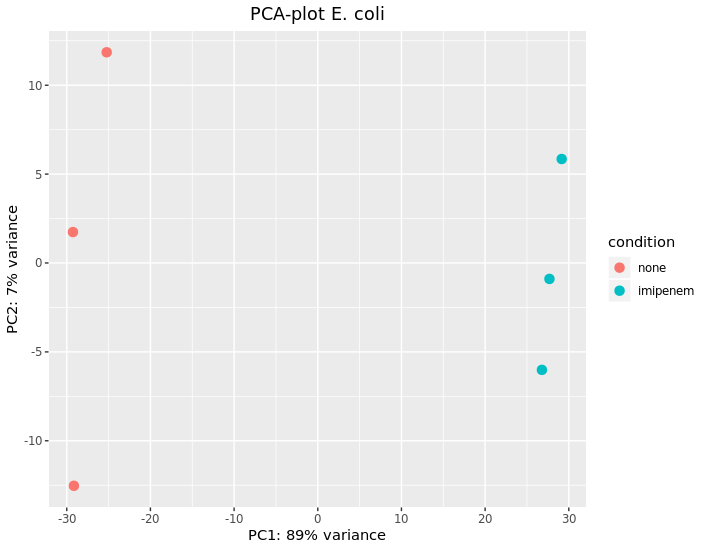
\includegraphics[width=0.9\linewidth]{Figures/PCA_E_coli2.png}
        \caption{PCA-plot \textit{E.coli}}
        \end{subfigure}
    \begin{subfigure}{0.47\textwidth}
        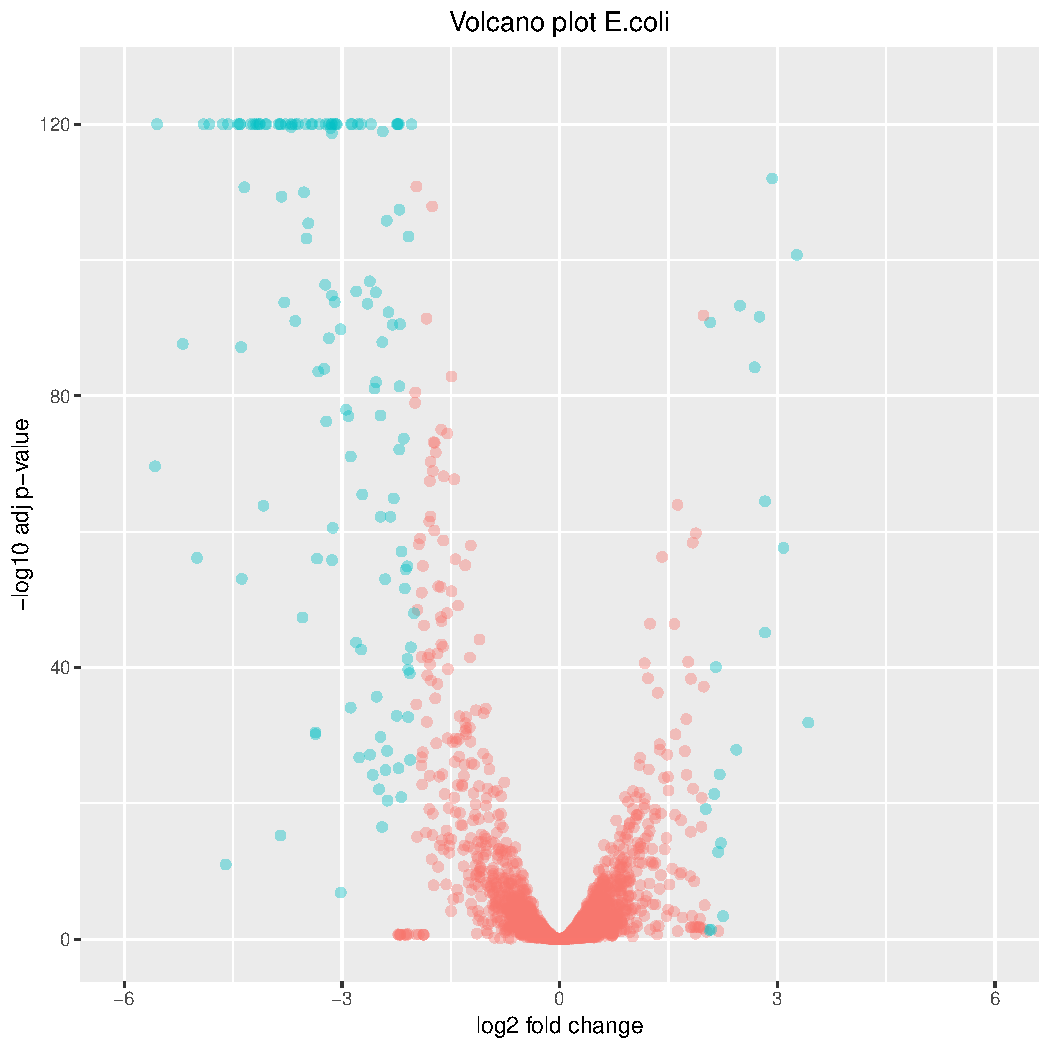
\includegraphics[width=0.9\linewidth]{Figures/Volcano_E_coli.pdf}
        \caption{Volcano plot \textit{E.coli}}
    \end{subfigure}
    \caption{PCA-plot of the six \textit{E.coli} samples (a), and a volcano plot over the deferentially expressed genes for \textit{E.coli} (b). The PCA-plot indicates that the majority of the variance between \textit{E. coli} samples can be explained by the first principal component. Samples "none" are controls while "imipenem" are the case samples. The blue objects in the volcano plot for \textit{E. coli} resembles the significant deferentially expressed genes with absolute $\mathrm{log}_2$ fold-change larger than $2$.}
    \label{fig:pca_volc_E_coli}
\end{figure}

% Table of top20 sign #5
The original study found 1563 out of 4550 significantly deferentially expressed genes in \textit{E. coli} with 765 up-regulated and 798 down-regulated genes \cite{jousset2018transcriptional}. In this study, 1520 out of 4521 genes were found significantly deferentially expressed, where 753 were up-regulated and 767 were down-regulated. The 20 most significant cases for each study are presented in table \ref{tabular:E.coli_diff_org}, respectively table \ref{tabular:E.coli_diff} in appendix A. Although the order is slightly different, the similarity between the findings is high. The p-values are of equal sizes and are remarkably small for both studies. The log fold-changes have the approximately same effect when comparing the same genes.

% Orginalstudien: Among differentially expressed genes, 154 RNAs had a Fold-Change (FC) >2 and 329 RNAs had a FC < 0.5. 


%----------------------------------------------------------------------------------------
%	Plasmid SECTION
%----------------------------------------------------------------------------------------
\subsection{Plasmid}
 % PCA #2
 In this study, a PCA-plot was also created based on the normalised plasmid samples. The first principal component explains 46\% of the variance, and the second principal component 31\%, as seen in figure \ref{fig:pca_volc_plasmid}a. The case samples are clearly separated from the controls in the plot. 

% Volcano #4or3
The genes studied in the differential expression analysis are plotted in a volcano plot in figure \ref{fig:pca_volc_plasmid}b. The significantly deferentially expressed genes (adj p-value$<$0.05) with absolute $\mathrm{log}_2$ fold-change $\geq 0.5$ are presented in blue. Genes to the right in the plot are up-regulated in the case samples while genes to the left are down-regulated.

\begin{figure}[ht]
    \centering
    \begin{subfigure}{0.47\textwidth}
        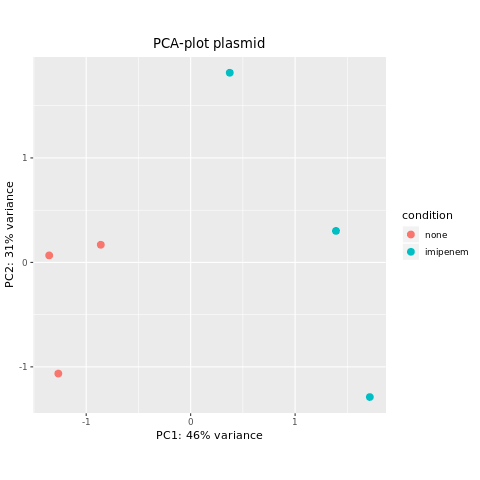
\includegraphics[width=0.9\linewidth]{Figures/PCA_plasmid.png}
        \caption{PCA-plot plasmid}
        \end{subfigure}
    \begin{subfigure}{0.47\textwidth}
        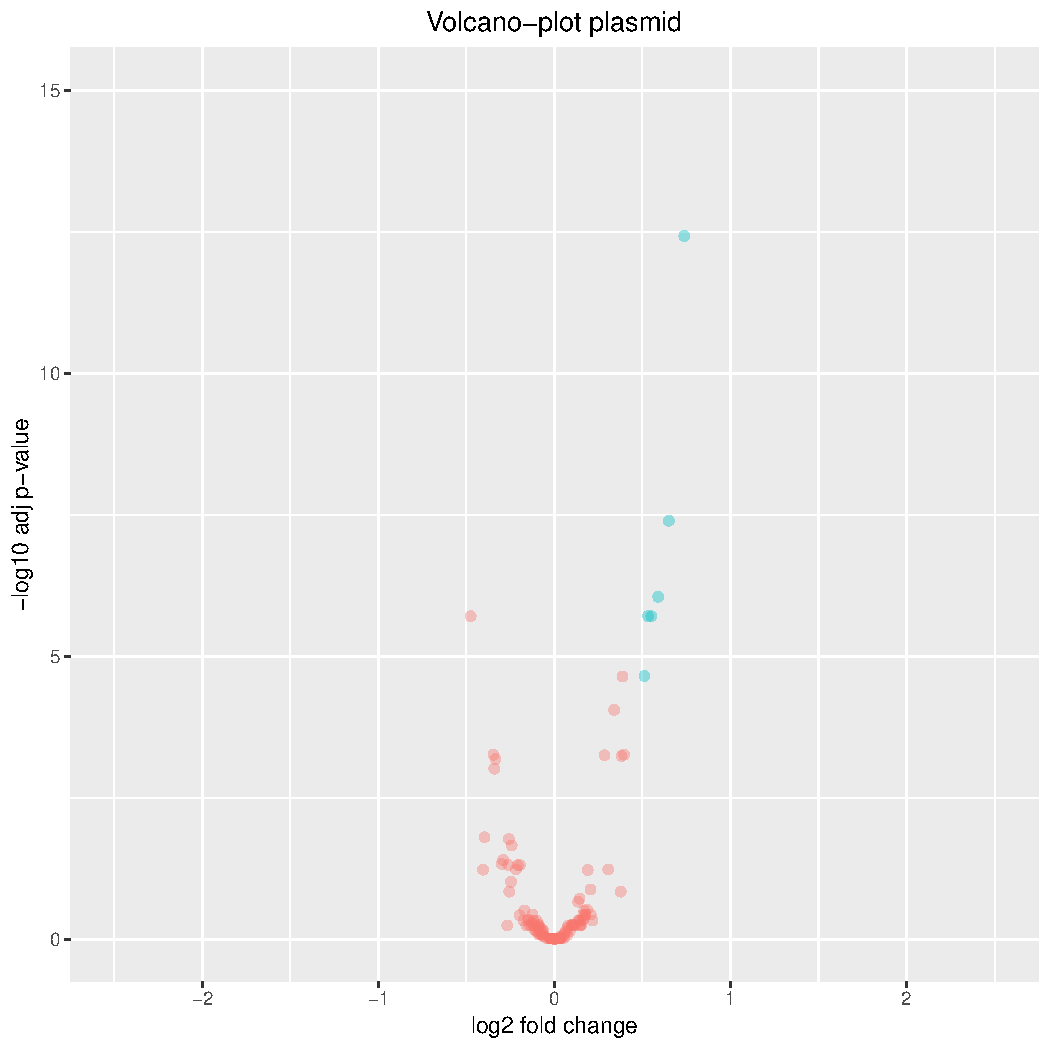
\includegraphics[width=0.9\linewidth]{Figures/Volcano_Plasmid.pdf}
        \caption{Volcano plot plasmid}
    \end{subfigure}
    \caption{PCA-plot of the six plasmid samples (a), and a volcano plot over the differentially expressed genes for the plasmid (b).The PCA-plot indicates that the majority of the variance between plasmid samples can be explained by the first and second principal components. Condition "none" correspond to the control samples and "imipenem" to the case samples. The blue objects in the volcano plot for the plasmid resemble the significantly differentially expressed genes with absolute $\mathrm{log}_2$ fold-change larger than $0.5$.}
    \label{fig:pca_volc_plasmid}
\end{figure}

% Table of sign #5
 The original report found 28 out of 193 significantly deferentially expressed genes in the plasmid where 9 were up-regulated and 19 down-regulated \cite{jousset2018transcriptional}. In this study, 23 out of 204 were found significantly differentially expressed, where 12 were up-regulated and 11 down-regulated. The significant cases for each study are presented in table \ref{tabular:plasmid_diff_org}, respectively table \ref{tabular:plasmid_diff} in appendix B. In general the p-values and log fold changes are of equal sizes for both studies. For example, in the original study, none of the genes had an absolute $\mathrm{log}_2$ fold change above two, which our findings also reflect, see figure \ref{fig:pca_volc_plasmid}b. 
 
 The accessible data of the plasmid lacked the gene names, which results in the comparison between the two studies being less exact. However, by instead comparing the descriptions of the genes in the two studies as well as their effect sizes and p-values, it can be concluded that many of the significant genes have similar functions and effects. It can be assumed that some of the significantly differentially expressed genes in respective study are the same, such as the most significant gene in both studies (pBIC\_0008 and CHX41\_27865).

\newpage
\section{Discussion}
%Compare our results with original\\
%Possible reasons for differences, felkällor\\

%Diskutera att det är okej att använda tidigare version av Bowtie eftersom våra reads inte är så långa



%CHECK Färre totalt antal gener (40), redan från countmatrix (början) 

%CHECK Gff filen kan innehålla färre gener --> färre annoterade gener, men samma gff fil som användes i artikeln.

%CHECK Kan ha att göra med nyare DSEq version.

% Några toppgener stämmer överens, men inte alla. Några saknas. Några är version 1 och två, saknad kunskap? Annan 

%CHECK ingen normalisering rekommenderad i artikel för PCA, körde på rekommenderade av DSEq --> Samma tolkning men annan PCA plot. Misstänkt anledning till annat utseende på PCA plot
The purpose of reproducing the results from the study was partially successful. Although the results were overall similar, some information differed in number of expressed genes and the plasmid annotation was unsuccessful, making it hard to compare results.  

In \textit{E.coli}, the 20 most significant differentially expressed genes, see tables \ref{tabular:E.coli_diff_org} and \ref{tabular:E.coli_diff}, are similar between the original study and the reproduction. The gene \textit{deuC} seems to be split in two genes in the original study, \textit{deuC\_1} and \textit{deuC\_2}. The gff-file used is from the original study, but the resulting amount of genes from the annotation differs. This could be because the annotation in process differs between the studies, due use of a later versions of genomicFeatures and genomicAlignments or due to difference in information.  Furthermore, there is a difference in the order of significance of the top significant genes, possibly due to use of different DESeq versions.

The PCA plots differ somewhat between the original study and the reproduction of it (see figures \ref{fig:orig_study_figures} and \ref{fig:pca_volc_E_coli}). It is possible that the reason for this is a difference in normalisation methods. No normalisation method was mentioned in the article and therefore the method used for this study was the one recommended for DESeq.

However, when comparing the results for the \textit{E. coli} genome, from the original study to the results of this study, the PCA and volcano plots, in figures \ref{fig:orig_study_figures} and \ref{fig:pca_volc_E_coli}, are similar and the tables \ref{tabular:E.coli_diff_org} and \ref{tabular:E.coli_diff}, of the most significantly deferentially expressed genes, although ordered differently, contain many of the same genes. Thus, one can conclude that the reproduction of this part has succeeded. 


%PLASMID

%CHECK Signifikanta plasmidgeners annotering i table 4 finns inte någon annanstans. Stämmer inte överens med gener i plasmiden på ncbi, inte heller beskrivning hittas --> Vi kan ej annotera vårå plasmigener på samma sätt, så vi kan ej jämföra. Fold change verkar stämma men vi kan ej bekräfta identitet.


As for the result of the plasmid analysis, the annotation of the genes found in table \ref{tabular:plasmid_diff_org} have not been found in NCBI's version of the plasmid, nor anywhere else. Thus the genes could not be annotated, making it impossible to compare the results for the differentially expressed genes from the original study to the results of the reproduction (see tables \ref{tabular:plasmid_diff_org} and \ref{tabular:plasmid_diff}). When comparing the tables further, the fold changes of gene expression in the original and reproduction study seem similar, indicating that reproduction could be successful. However, this can not be confirmed as the gene identities remain unknown. It should be noted that with a low plasmid gene expression, a bigger sample size would be needed to detect differences. Thus, it is possible that repeating the study with a larger sample size might lead to different results due to increased power of the tests. 

% SÄG NÅGOT OM FIGUR 3

%The study could be made more clear an specific as to what was done and how, in every step of the way.
%In conclusion --- how reproducible was the study?????
When compared, the reproduction of the study provided results rather similar to the original study. However, the original study could have been more clear and detailed. As an example, the normalization method for PCA was not mentioned, resulting in a different a different mapping even if the overall result was the same. A major defect of the study was the inability of confirming the plasmid gene annotations, making it impossible to compare the results. An addition of further information about points such as these would improve the article, as it can be concluded that reproduction of the study was not fully possible.



%Bowtie comparison 
%Bowtie-0.12.7 differs from the latest version, but comparison was found of these specifically. The closest comparison was that of Bowtie 1 and Bowtie 2 \cite{bowtie}, where the biggest difference was that Bowtie 2 is able to process longer reads compared to Bowtie 1, whilst Bowtie 1 should perform equally well for sequence reads under ~50 bp. Furthermore, the present version has an increased throughput rate and fully supports gapped alignments, which bowtie 1 does not. 

%\section{Appendix}


% List of references 
\newpage
\bibliographystyle{vancouver}
\bibliography{References.bib}

% Reference through \cite{mensh2017ten}

\newpage
\appendix
\section{Differentially expressed genes in \textit{E. coli}}

\begin{table}[ht]
\centering
\caption{The 20 most significantly deferentially expressed genes in \textit{E. coli} found in the original study. The genes are ordered in descending order according to significance.}
\footnotesize
\begin{tabular}{lcccl}
  \hline
 gene& log2\_fold\_change & fold\_change & padj& Annotation \\ 
  \hline
  dcuC\_1&	-4.3&5.0E-02	&	0&	anaerobic C4-dicarboxylate transport\\
glpA	&-5.6	&2.1E-02&	0&	sn-glycerol-3-phosphate dehydrogenase, large subunit\\
yfcC	&-5.1&2.8E-02&	0&	predicted inner membrane protein\\
yhbU	&-4.8&3.6E-02	&	0&	predicted peptidase\\
nikB	&-4.6&4.1E-02&	0&	nickel transporter subunit; membrane comp. of ABC superfamily\\
nikC	&-4.5&4.4E-02&	0&	nickel transporter subunit; membrane comp. of ABC superfamily\\
frdC	&-3.8&7.0E-02	&	0&	fumarate reductase, membrane anchor subunit\\
frdA    &-3.6	&8.1E-02	&	0&	fumarate reductase catalytic and NAD/flavoprotein subunit\\
yhbV	&-3.9&6.6E-02	&	2.7E-302&	predicted protease\\
gatY	&-3.4&9.4E-02	&	2.4E-297&	D-tagatose 1,6-bisphosphate aldolase 2, catalytic subunit\\
aspA	&-3.2&1.1E-01	&	4.2E-292&	aspartate ammonia-lyase\\
dcuC\_2	&-4.2&5.3E-02	&	1.2E-289&	anaerobic C4-dicarboxylate transport\\
yjjI	&-4.8&3.6E-02	&	6.9E-273&	conserved protein\\
nirD	&-3.3&1.0E-01	&	2.1E-270&	nitrite reductase, NAD(P)H-binding, small subunit\\
glpB	&-4.8&3.6E-02	&	5.8E-245&	sn-glycerol-3-phosphate dehydrogenase, membrane anchor subunit\\
napB	&-4.1&5.8E-02	&	1.5E-237&	nitrate reductase, small, cytochrome C550 subunit, periplasmic\\
nikE	&-4.2&5.3E-02	&	3.2E-234&	nickel transporter subunit; ATP-binding comp. of ABC superfamily\\
glpT	&-3.5&8.7E-02&	2.2E-227&	sn-glycerol-3-phosphate transporter\\
hybO	&-3.66&1.1E-01	&	9.1E-213&	hydrogenase 2, small subunit\\
yjjW	&-4.2&6.0E-02	&	1.1E-210&	predicted pyruvate formate lyase activating enzyme\\
  \hline
\end{tabular}
    \label{tabular:E.coli_diff_org}
\end{table}

\begin{table}[ht]
\centering
\caption{The 20 most significantly differentially expressed genes in \textit{E. coli} found in this study. The genes are ordered in descending order according to significance.}
\footnotesize
\begin{tabular}{lccc}
  \hline
 gene& log2\_fold\_change & fold\_change & padj \\ 
  \hline
dcuC & -4.1 & 6.0E-02 & 0 \\ 
  frdC & -3.8 & 7.0E-02 & 0 \\ 
  gatY & -3.4 & 9.3E-02 & 0 \\ 
  glpA & -5.5 & 2.1E-02 & 0 \\ 
  nikB & -4.4 & 4.7E-02 & 0 \\ 
  nikC & -4.4 & 4.6E-02 & 0 \\ 
  yfcC & -4.9 & 3.3E-02 & 0 \\ 
  yhbU & -4.6 & 4.0E-02 & 0 \\ 
  yhbV & -3.8 & 7.3E-02 & 0 \\ 
  yjjI & -4.2 & 5.4E-02 & 0 \\ 
  nirD & -3.3 & 1.0E-01 & 1.5E-287 \\ 
  frdA & -3.6 & 8.0E-02 & 1.8E-283 \\ 
  aspA & -3.1 & 1.1E-01 & 8.5E-277 \\ 
  glpB & -4.6 & 4.2E-02 & 3.4E-262 \\ 
  napB & -4.1 & 5.7E-02 & 3.8E-245 \\ 
  glpT & -3.5 & 8.8E-02 & 4.2E-243 \\ 
  hybO & -3.1 & 1.1E-01 & 3.2E-217 \\ 
  yjjW & -3.9 & 6.9E-02 & 1.2E-201 \\ 
  frdD & -3.9 & 6.8E-02 & 2.2E-194 \\ 
  napC & -3.2 & 1.1E-01 & 1.4E-189 \\ 
   \hline
\end{tabular}
    \label{tabular:E.coli_diff}
\end{table}

\newpage

\section{Differentially expressed genes pBIC-1a plasmid}

\begin{table}[ht]
\centering
\caption{The 28 significantly differentially expressed genes in the plasmid found in the original study. The genes are ordered in descending order according to significance.}
\footnotesize
\begin{tabular}{lcccl}
  \hline
    gene &  log2\_fold\_change & fold\_change & padj & Description \\ 
  \hline
    pBIC\_00008 & -1.28&	0.41&	1.2E-13&	Transposase (ISKpn6)\\
    pBIC\_00007	&-1.15	&0.45&	5.0E-12&	Transposase DDE domain protein\\
    pBIC\_00172 &	-0.68 &	0.62 &	1.5E-08 &	Helix-turn-helix domain protein\\
    pBIC\_00108 &	-1.22 &	0.43 &	4.9E-08	& Hypothetical protein\\
    hspA\ &	-0.58 &	0.67 &	4.4E-07 &	Heat shock protein\\
    pBIC\_00098 &	-1.03 &	0.49 &	5.3E-07	& Helix-turn-helix domain protein\\
    pBIC\_00097 &	-0.66 &	0.64 &	6.4E-06	& Putative transposase\\
    yjcC &	-0.58 &	0.67 &	7.7E-06 & Putative membrane protein YjcC\\
    pBIC\_00034 &	-0.43 & 0.74 &	3.2E-05	& Conjugal transfert protein TraG\\
    mepM &	0.46 &	1.37 &	1.9E-04 &	Murein DD-endopeptidase MepM\\
    pBIC\_00168 &	-0.43 &	0.74 &	2.0E-04	& Diguanylate cyclase\\
    clpC &	-0.41 &	0.75 &	2.2E-04	& ATP-dependent Clp protease ATP-binding subunit ClpC\\
    pBIC\_00069 &	-0.37& 	0.77 &	8.5E-04	& Hypothetical protein\\
    pBIC\_00176	& -0.51	& 0.70 &	1.8E-03	& Transposase (ISKpn26)\\
    pBIC\_00107	& 0.94 &	1.91 &	3.2E-03 &	Transposase\\
    copA &	0.33 &	1.25 &	3.4E-03 &	Copper resistance protein A precursor\\
    copD &	0.31 &	1.24&	8.3E-03&	Copper resistance protein D\\
    copS&	0.31&	1.24&	9.5E-03	&Sensor kinase CopS\\
    higA&	-0.28&	0.82&	1.4E-02&	Antitoxin HigA\\
    pBIC\_00006&	-0.52&	0.70&	1.9E-02&	Transposase (ISKpn31)\\
    copR&	0.25&	1.19&	2.4E-02	&Transcriptional activator protein CopR\\
    pBIC\_00169&	-0.34&	0.79&	2.7E-02	&Hypothetical protein\\
    pBIC\_00177&	-0.53&	0.70&	2.9E-02	&Hypothetical protein\\
    pcoE&	0.33&	1.26&	3.0E-02	&Putative copper-binding protein PcoE precursor\\
    copB&	0.37&	1.29&	3.5E-02	&Copper resistance protein B precursor\\
    pBIC\_00186& 	-0.39&	0.76&	4.0E-02&	Transposase (IS26)\\
    pBIC\_00064&	-0.24&	0.85&	4.7E-02	&Lytic Transglycosylase\\
    pBIC\_00010&	0.22&	1.17&	4.9E-02	&Hypothetical protein\\
   \hline
\end{tabular}
    \label{tabular:plasmid_diff_org}
\end{table}

\begin{table}[ht]
\centering
\caption{The 23 significantly differentially expressed genes in the plasmid found in this study. The genes are ordered in descending order according to significance.}
\footnotesize
\begin{tabular}{lcccl}
  \hline
 gene& log2\_fold\_change & fold\_change & padj & Description \\ 
  \hline
  CHX41\_27865 & -7.4E-01 & 0.60 & 3.8E-13 & transposase \\ 
  CHX41\_28220 & -6.5E-01 & 0.64 & 4.0E-08 & DNA-binding protein \\ 
  CHX41\_27925 & -5.9E-01 & 0.66 & 8.9E-07 & cyclic diguanylate phosphodiesterase \\ 
  CHX41\_28015 & 4.8E-01 & 1.40 & 2.0E-06 & peptidase M23 \\ 
  CHX41\_28200 & -5.3E-01 & 0.69 & 2.0E-06 & diguanylate cyclase \\ 
  CHX41\_28215 & -5.5E-01 & 0.68 & 2.0E-06 & Hsp20/alpha crystallin family protein \\ 
  CHX41\_27335 & -5.1E-01 & 0.70 & 2.2E-05 & ISAs1 family transposase \\ 
  CHX41\_27480 & -3.9E-01 & 0.76 & 2.3E-05 & conjugal transfer protein TraG \\ 
  CHX41\_27685 & -3.4E-01 & 0.79 & 8.9E-05 & addiction module toxin RelE \\ 
  CHX41\_28025 & 3.5E-01 & 1.30 & 5.5E-04 & copper resistance protein A \\ 
  CHX41\_28195 & -4.0E-01 & 0.76 & 5.5E-04 & diguanylate cyclase \\ 
  CHX41\_27680 & -2.8E-01 & 0.82 & 5.6E-04 & XRE family transcriptional regulator \\ 
  CHX41\_28210 & -3.8E-01 & 0.77 & 5.8E-04 & ATP-dependent Clp protease ATP-binding subunit \\ 
  CHX41\_28050 & 3.3E-01 & 1.3 & 6.6E-04 & sensor histidine kinase \\ 
  CHX41\_28040 & 3.4E-01 & 1.3 & 9.7E-04 & copper resistance protein D \\ 
  CHX41\_28030 & 4.0E-01 & 1.3 & 1.6E-02 & copper resistance protein B \\ 
  CHX41\_28045 & 2.6E-01 & 1.2 & 1.7E-02 & DNA-binding response regulator \\ 
  CHX41\_27350 & 2.4E-01 & 1.2 & 2.2E-02 & hypothetical protein \\ 
  CHX41\_28055 & 2.9E-01 & 1.2 & 4.0E-02 & copper-binding protein \\ 
  arsH & 3.0E-01 & 1.2 & 4.7E-02 & arsenical resistance protein ArsH \\ 
  CHX41\_27345 & 2.0E-01 & 1.1 & 4.9E-02 & carbapenem-hydrolyzing class A beta-lactamase KPC-2 \\ 
  CHX41\_28035 & 2.6E-01 & 1.2 & 4.9E-02 & copper resistance protein CopC \\ 
  CHX41\_28160 & 2.1E-01 & 1.2 & 4.9E-02 & hypothetical protein \\ 
   \hline
\end{tabular}
    \label{tabular:plasmid_diff}
\end{table}



%% Samlar lite saker här som vi eventuellt vill ha med i appendixet, alternativt ta bort helt.

% Heat map E.coli #1
\textcolor{blue}{Should this be in the discussion?}\\
By creating a heat map of the Poisson distances between the \textit{E. coli} samples, the relation between the six studied samples could be verified. The heat map is presented in figure \ref{fig:E.coli_pois} and shows two clear clusters that group case samples in one cluster and control samples in the other cluster.  \textcolor{blue}{This was as expected.} The colour intensity increases as the distance decreases, which indicates a higher resemblance between samples. \textcolor{blue}{Poisson distances were used instead of Euclidean distances, since/because ...}

\begin{figure}[ht]
    \centering
    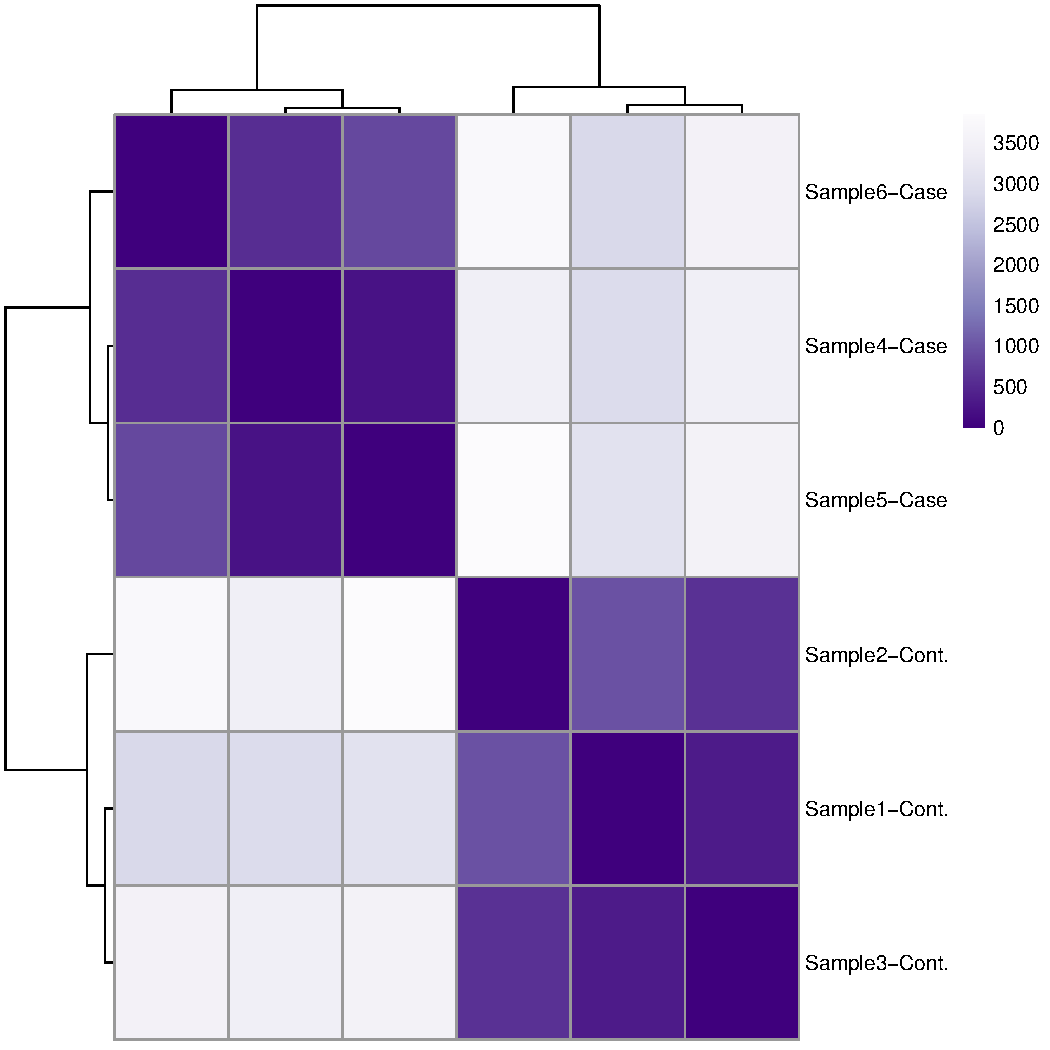
\includegraphics[scale=0.6]{Figures/Pois_dist_heat_E_coli.pdf}
    \caption{The Poisson distances between \textit{E. coli} samples visualised by colour intensity. Samples are clustered according to resemblance.}
    \label{fig:E.coli_pois}
\end{figure}
 
 % Histogram E.coli #3or4
The p-values obtained from the differential expression analysis of \textit{E. coli} are plotted in a histogram in figure \ref{fig:E.coli_hist}. The distribution is approximately uniform for p-values $>$ 0.05. \textcolor{blue}{This is good since the assumption is that p-values are uniformly distributed under the null hypothesis and that they are $<$ 0.05 when the null hypothesis is rejected.}

\begin{figure}[h!]
    \centering
    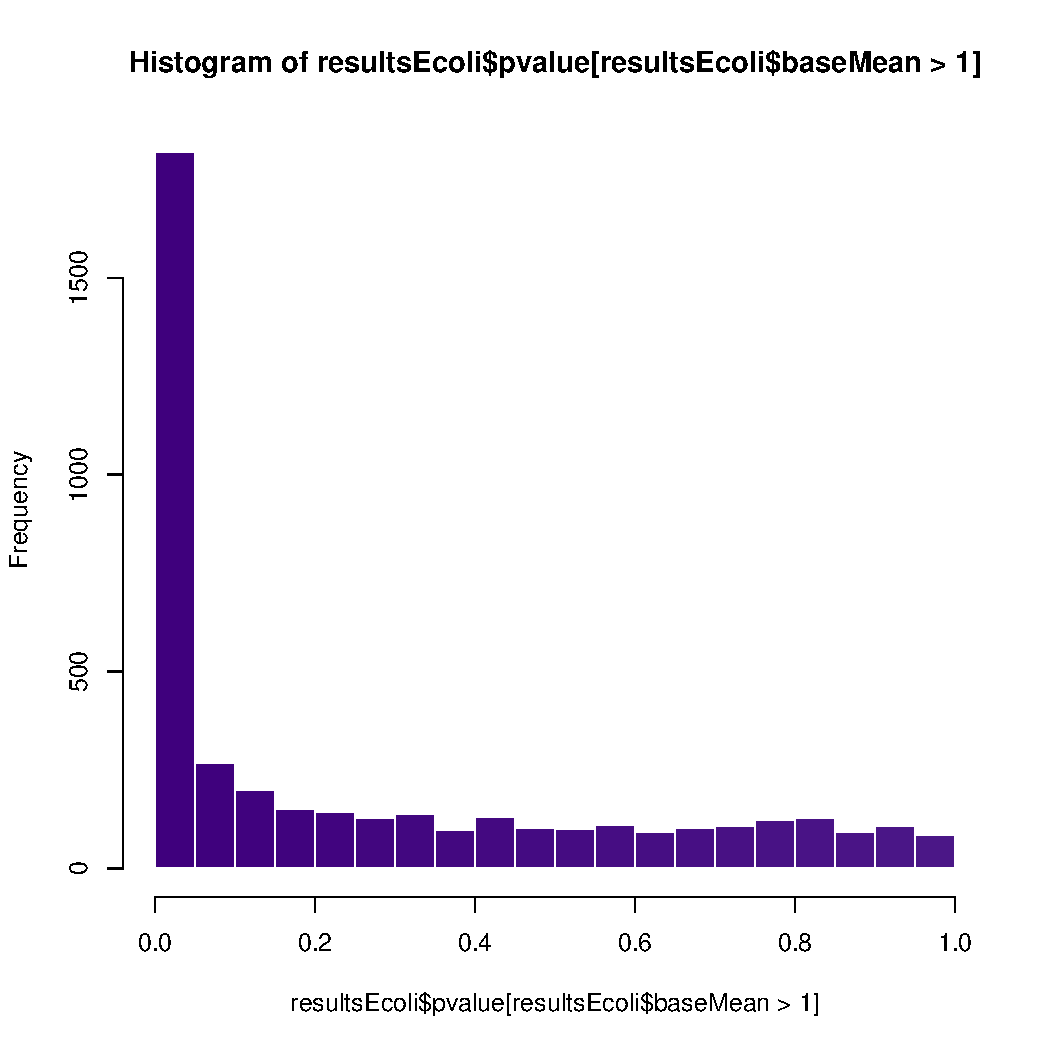
\includegraphics[scale=0.5]{Figures/Histogram_pvalues_E_coli.pdf}
    \caption{The histogram of p-values obtained for genes expressed in \textit{E. coli}. The distribution is approximately uniform for p-values $>$ 0.05. }
    \label{fig:E.coli_hist}
\end{figure}

% heat map plasmid #1
The heat map created for Poisson distances between the plasmid samples is presented in figure \ref{fig:plasmid_hist} and shows a clear cluster which groups the control samples together. The case samples are also grouped together, although their Poisson distances is larger, as seen in the figure by the lighter colour. This indicates that they are less similar than the control samples. \textcolor{blue}{The heat map was as expected. Compared to the heat map created for the \textit{E. coli} samples, this heat map shows larger resemblance between all samples and less defined clusters, which could be due to lower gene expression for the plasmid and thus fewer gene counts in the samples.}
\begin{figure}[h!]
    \centering
    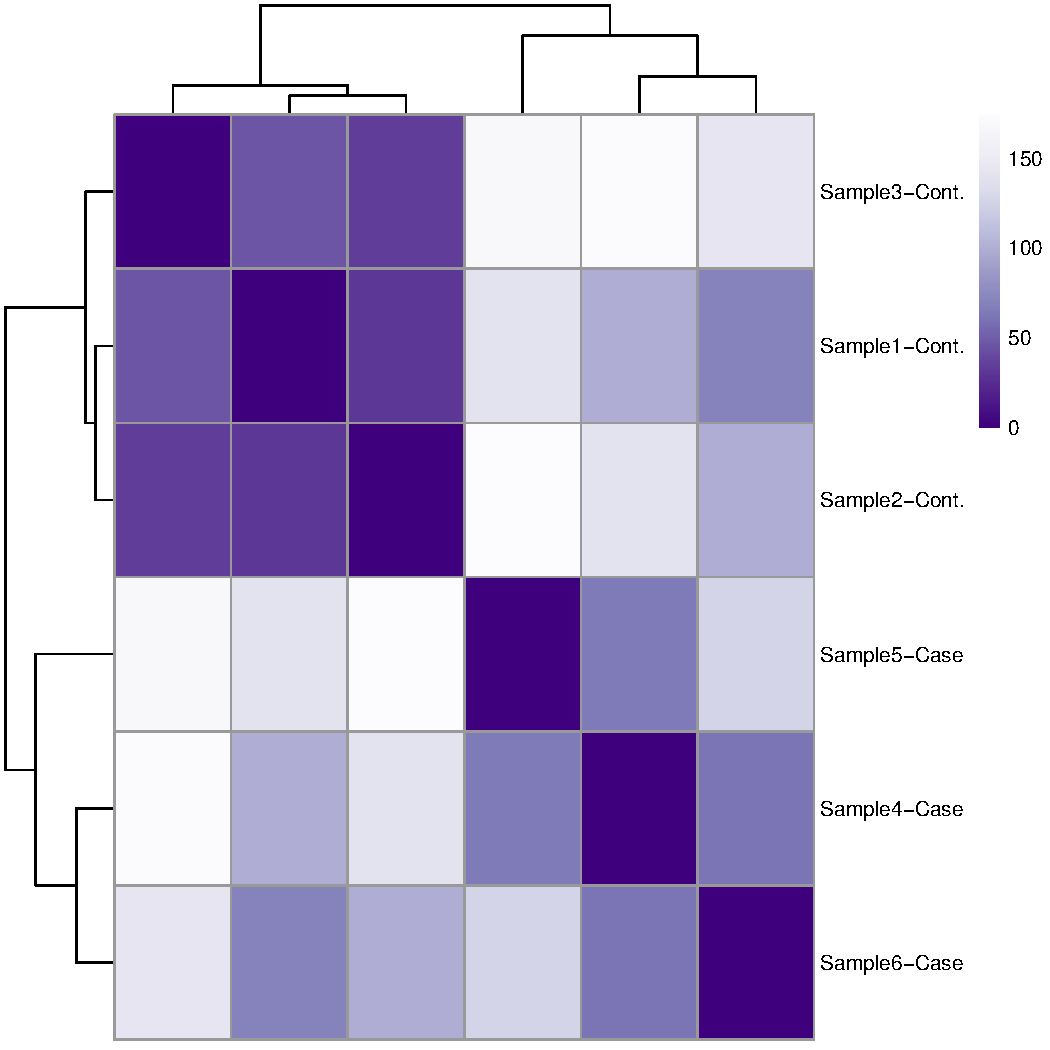
\includegraphics[scale=0.6]{Figures/Pois_dist_heat_plasmid.pdf}
    \caption{The Poisson distances between plasmid samples visualised by colour intensity. Samples are clustered according to resemblance.}
    \label{fig:plasmid_pois}
\end{figure}

% Histogram plasmid #3or4
The p-values obtained from the differential expression analysis of the plasmid are plotted in a histogram in figure \ref{fig:plasmid_hist}. The distribution is roughly uniform for p-values $>$ 0.05. 
\begin{figure}[h!]
    \centering
    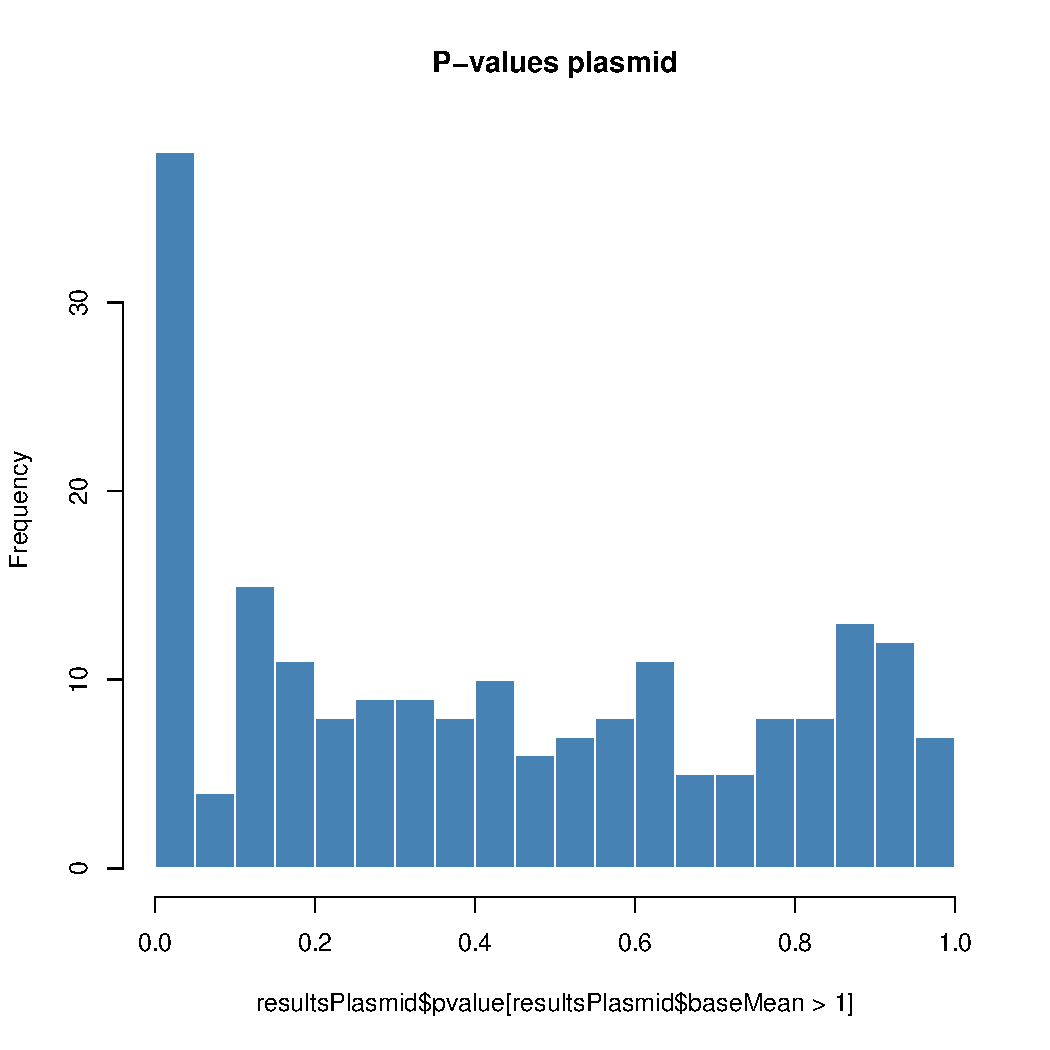
\includegraphics[scale=0.5]{Figures/Histogram_pvalues_plasmid.pdf}
    \caption{The histogram of p-values obtained for genes expressed in the plasmid. The distribution is roughly uniform for p-values $>$ 0.05.}
    \label{fig:plasmid_hist}
\end{figure}
 


\end{document}

